\section{Navigation}
\label{sec:navigation}
I implementeringen af rutenavigation måtte forskellige kortest-vej algoritmer overvejes. En passende algoritme til formålet måtte udnytte en graf over kortdataet, som blev genereret under opstart. Derudover måtte algoritmen også kunne inddrage faktorer som længden eller hastighedsgrænsen af et vejsegment i dennes vurdering af den optimale rute. Da vi ønskede at opfylde det udvidede krav til rutenavigation, om at destinationen skulle kunne ændres kontinuerligt og flydende, var det naturligt at anvende en algoritme, som genererer et kortest-vej træ. Med et sådant træ er det nemlig muligt at udvinde den korteste vej fra træets startknude og til enhver anden knude i grafen med konstant tid.

\subsection{Dijkstra}
\label{subsec:dijkstra}
Sådanne kortest-vej træs algoritmer trumfes af E. W. Dijkstras grafsøgningsalgoritme. Dijkstras algoritme tager udgangspunkt i en startknude hvorfra det resterende træ genereres. Hver af dennes tilstødende knuder besøges. Et besøg består i at sammenholde den kendte afstand mellem startknuden og den besøgte med den nye afstand. Den nye afstand ses som den kendte afstand mellem startknuden og den besøgende knude sammenlagt med afstanden mellem den besøgende og den besøgte knude. Har en knude aldrig været besøgt, er afstanden til denne blot angivet som $+\infty$, hvorfor ethvert nyt forslag er en forbedring. Besøgsrækkefølgen varetages af en prioritetskø, som prioriterer de tilstødende knuder med lavest afstand til startknuden højest.

\begin{figure}[h]
	\centering
  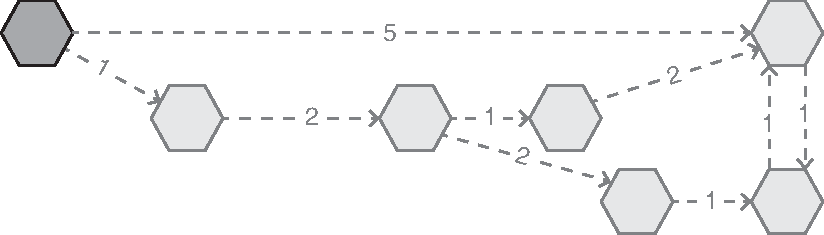
\includegraphics[width=0.9\textwidth]{dijkstra1}
  \captionsetup{width=0.8\textwidth}
  \caption{Eksempel på en vægtet orienteret graf.}
\end{figure}

\begin{figure}[h]
	\centering
  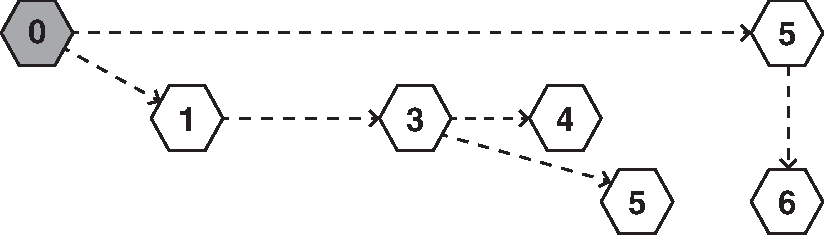
\includegraphics[width=0.9\textwidth]{dijkstra2}
  \captionsetup{width=0.8\textwidth}
  \caption{Det resulterende kortest-vej træ med udgangspunkt i den grønne startknude. Distancen mellem de individuelle knuder og startknuden ses angivet.}
\end{figure}

\subsection{A*}
\label{subsec:astar}
En anden algoritme, som blev inddraget i overvejelserne, var A*-algoritmen. Denne generer ikke, ligesom Dijkstras, et kortest-vej træ, men finder blot den korteste vej mellem en given start- og slutknude. Da A* udvider funktionaliteten af Dijkstras algoritme, er deres adfærd meget tilsvarende. Hvor Dijkstras blot iagttager den traverserede afstande mellem den besøgte knude og startknuden, vurderer A* også en heuristik $h(x)$ for afstanden til \emph{slutknuden}. Besøgsrækkefølgen varetages stadigvæk af en prioritetskø, men nu prioriteres der efter funktionen $f(x)=g(x)+h(x)$, hvor $g(x)$ er afstanden mellem den besøgte knude og startknuden som set i Dijkstras.

\begin{figure}[h]
	\centering
  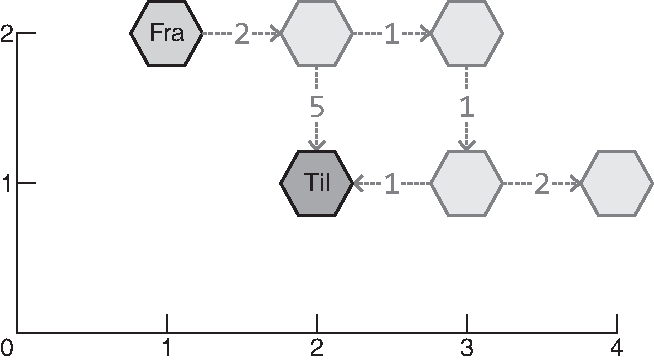
\includegraphics[width=0.9\textwidth]{astar1}
  \captionsetup{width=0.8\textwidth}
	\caption{A picture of a gull.}
\end{figure}

\begin{figure}[h]
	\centering
  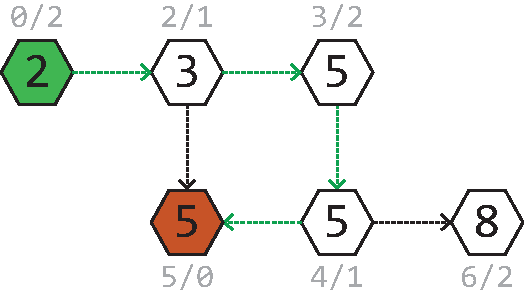
\includegraphics[width=0.9\textwidth]{astar2}
  \captionsetup{width=0.8\textwidth}
	\caption{A picture of a gull.}
\end{figure}

\subsection{Ruteomkostninger}
\label{subsec:ruteomkostninger}
%længde = tid
%valg af heuristik